\documentclass[tikz,border=8pt]{standalone}
\usepackage[T1]{fontenc}\usepackage{lmodern,amsmath,amssymb}\usetikzlibrary{arrows.meta,positioning}
\begin{document}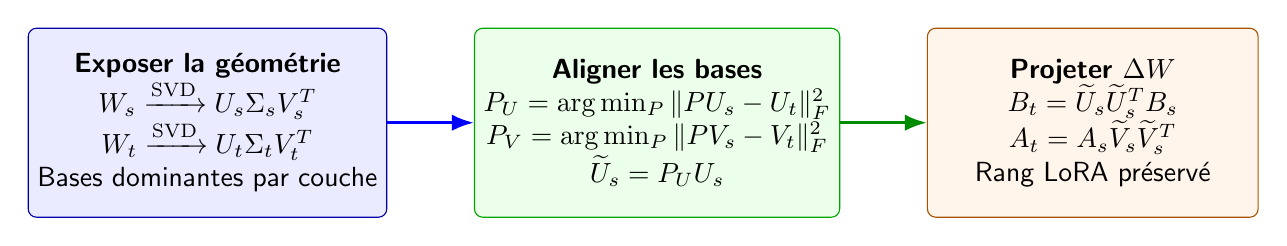
\begin{tikzpicture}[font=\sffamily,>=Latex,node distance=11mm,box/.style={draw=#1!65!black,fill=#1!8,rounded corners=3pt,minimum width=4.2cm,minimum height=2.4cm,align=center},arr/.style={-{Latex},line width=1.1pt}]
\node[box=blue] (geo) {\textbf{Exposer la géométrie}\\$W_s\xrightarrow{\mathrm{SVD}}U_s\Sigma_sV_s^T$\\$W_t\xrightarrow{\mathrm{SVD}}U_t\Sigma_tV_t^T$\\Bases dominantes par couche};
\node[box=green,right=of geo] (align) {\textbf{Aligner les bases}\\$P_U=\arg\min_P\|PU_s-U_t\|_F^2$\\$P_V=\arg\min_P\|PV_s-V_t\|_F^2$\\$\widetilde U_s=P_UU_s$};
\node[box=orange,right=of align] (proj) {\textbf{Projeter $\Delta W$}\\$B_t=\widetilde U_s\widetilde U_s^TB_s$\\$A_t=A_s\widetilde V_s\widetilde V_s^T$\\Rang LoRA préservé};
\draw[arr,blue] (geo)--(align);\draw[arr,green!55!black] (align)--(proj);
\end{tikzpicture}\end{document}
